\documentclass[vecarrow]{svproc}
% % RECOMMENDED  % to typesetURLs, URIs, and DOIs
\usepackage{url}
\def\UrlFont{\rmfamily}

\usepackage{listings}
\usepackage{color}
\definecolor{dkgreen}{rgb}{0,0.6,0}
\definecolor{gray}{rgb}{0.5,0.5,0.5}
\definecolor{mauve}{rgb}{0.58,0,0.82}
\lstset{frame=tb,
 aboveskip=3mm, belowskip=3mm,
showstringspaces=false, columns=flexible,
basicstyle={\small\ttfamily}, numbers=none,
numberstyle=\tiny\color{gray}, keywordstyle=\color{blue},
commentstyle=\color{dkgreen},
stringstyle=\color{mauve}, breaklines=true,
breakatwhitespace=true, tabsize=3 }

\usepackage{graphicx}

\usepackage{booktabs}

\usepackage{rotating}

\usepackage{pdflscape}

%\usepackage{amsmath}

\begin{document}
\mainmatter % start of a contribution %

\title{RNN in  tensorflow} %

\titlerunning{RNN in ensorflow}
% abbreviated title (for running head)
% also used for the TOC unless
% \toctitle is used %
\author{Mohd Zamri Murah} %
%\authorrunning{Ivar Ekeland et al.} % abbreviated author list (for running head)
% list of authors for the TOC (use if author list has to be modified)
%\tocauthor{Ivar Ekeland, Roger Temam, Jeffrey Dean, David
 \institute{Center for Artificial Intelligence
Technology\\ Fakulti Teknologi Sains
Maklumat\\ Universiti Kebangsaan Malaysia\\
\email{zamri@ukm.edu.my}}

\maketitle % typeset the title of the contribution

\begin{abstract}

Tensorflow is an open-source
deep learning library developed by Google.
It has been used in many areas such as image recognition, text
to speech engine, pattern recognition and
big data. This note provide an introductory concepts for
computation using tensorflow.

\keywords{deep learning}

\end{abstract} %

\section{Introduction}

Feed-forward networks operate on fixed size vectors. For example, they map the pixels of $28x28$ image to the probabilities of $10$ possible classes. The computation happens in a fixed number of steps, namely the number of layers. In contrast, recurrent networks can operate on variable length sequences of vectors, either as input, output or both.

RNNs are basically arbirary directed graphs of neurons and weights. Input neurons have
on incoming connections because their activation is set by the input data anyway. The
output neurons are just set of neurons in the graph that we read the prediction from. All
other neurons in the graph are referred to as hidden neurons.



A basic RNN is shown in
figure~\ref{fig:1}. 

\begin{figure}
% https://en.wikibooks.org/wiki/LaTeX/Importing_Graphics
% Use the relevant command to insert your figure file.
% For example, with the graphicx package use
\centering{\fbox{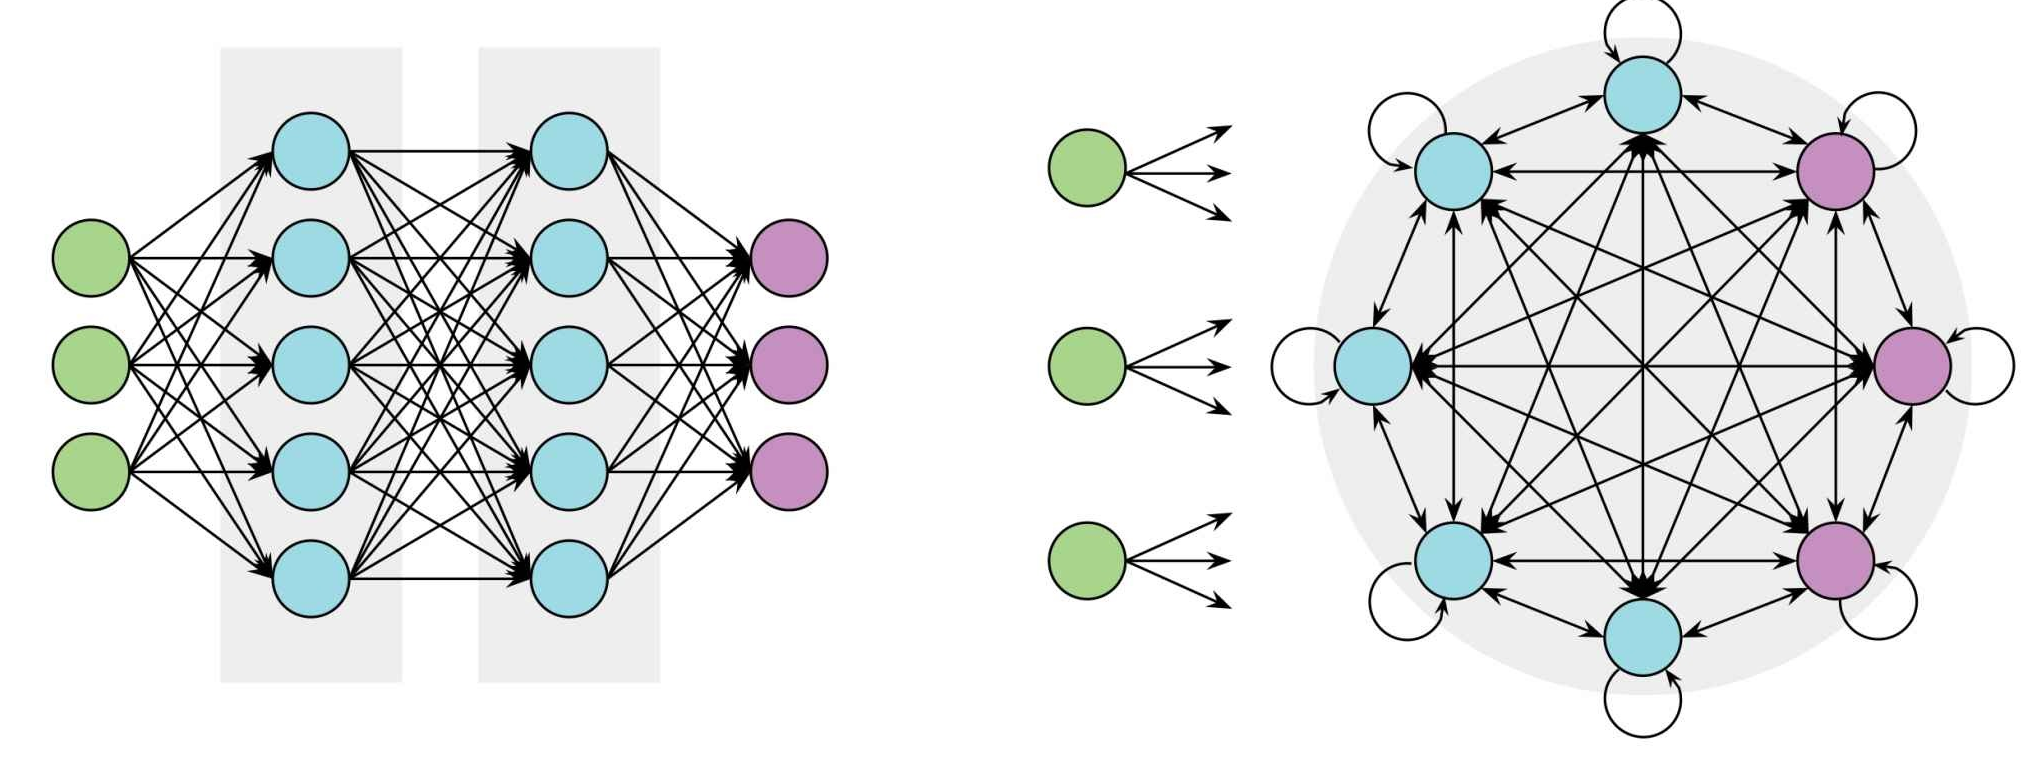
\includegraphics[scale=.15]{rnn.png}}} %
\caption{A feed-forward network and a recurrent network}
\label{fig:1}
% Give a unique label
\end{figure}

The state of an RNN depends on the current input and the previous state, which in turn
depends on the input and state before that. Therefore, the state has indirect access to all previous inputs of the sequence and can be interpreted as a working memory.

\begin{figure}
% https://en.wikibooks.org/wiki/LaTeX/Importing_Graphics
% Use the relevant command to insert your figure file.
% For example, with the graphicx package use
\centering{\fbox{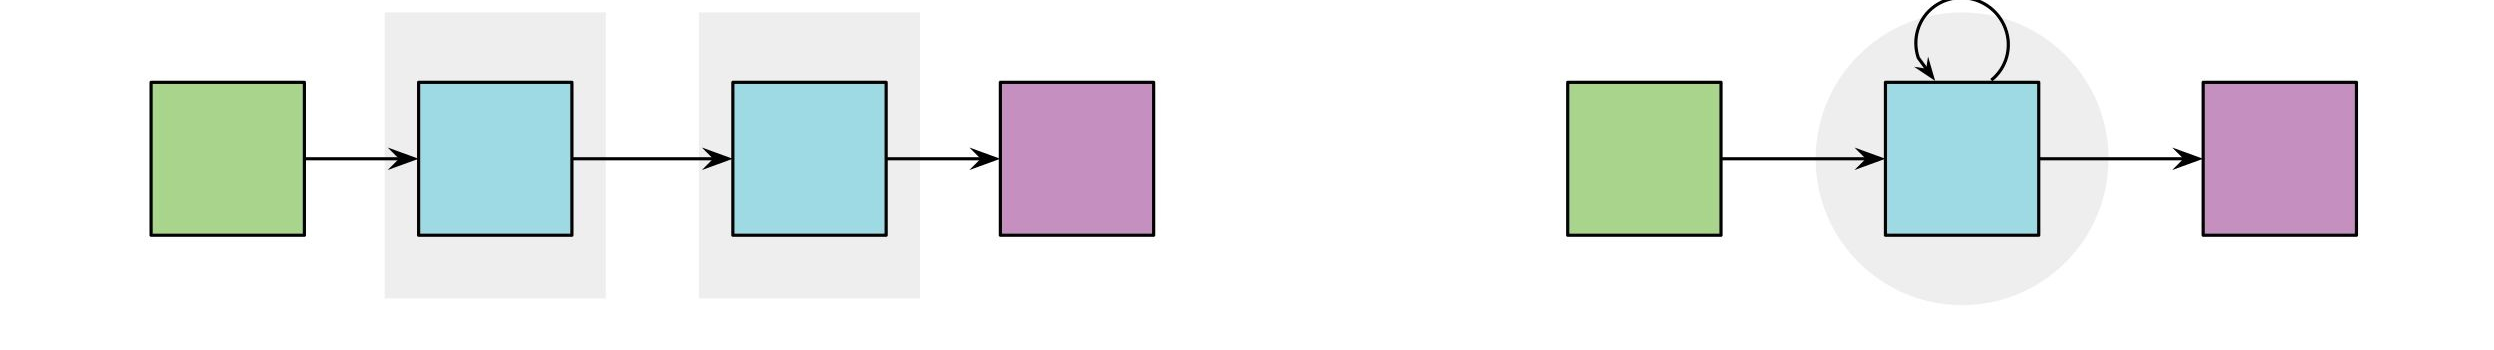
\includegraphics[scale=.15]{rnn1.png}}} %
\caption{A feed-forward network and a recurrent network}
\label{fig:1}
% Give a unique label
\end{figure}


\bibliography{tensorflow}
\bibliographystyle{splncs_srt}
\end{document}
